\documentclass{article}
\usepackage[utf8]{inputenc}
\usepackage{hyperref}
\usepackage{graphicx}
\graphicspath{ {./images/} }

\title{Journal#3 - Survey Paper Research}
\author{James A Turner}
\date{September 2022}
\maketitle

\begin{document}
\newpage
\section{Survey Notes/Critical Read}
\subsection{Article 1: Overview of Spectrum Sharing and Dynamic Spectrum Allocation Schemes in Cognitive Radio Networks(Most Recent}\cite{1}
The article provides a brief overview on current spectrum sharing techniques that cognitive radios use to provide efficient spectrum access for radio networks.  The overview is surface thin but provides enough to understand some basic algorithms and techniques used when deciding how devices will communicate in the radio spectrum.  It does provide enough entry level understanding of the pros and cons between different models.  It doesn't provide a good overview or cite other research into this area so there is no compare and contrast between taxonomies and methodologies.
\subsection{Article 2 A Review on SDR, Spectrum Sensing, and CR-based IoT in Cognitive Radio Networks}\cite{2}
This article was a comprehensive study and overview of cogntive radio networks and their functions.  The authors did an excellent job at providing current research on the topic and provided a cohesive taxonomy for the current study and research of cognitive radios.  This taxonomy largely revolves around spectrum sensing techniques, spectrum access techniques, decision-making cycle, and architecture.  The authors were careful to describe limitations and advantages that exist with each of the spectrum techniques and described current limitations and challenges with the technology.
\subsection{Article 3 Cognitive Radio Networks: A Survey}\cite{3}
The authors didn't go into as much detail as article 2, but they summarized and clarified the categories of research more efficiently and succinctly.  In addition, they added limitations to each section of the research, whereas the second article only covered generalizations in the field.  This style allowed for a more focused reading.
\subsection{Article 4 Cognitive Radio Spectrum Sensing: A Survey}\cite{4}
This article didn't go in as much detail as either article or two or three but generally followed the same classification of topics and concepts.  This article did provide a "future work" section that did spur some more thought into some of the issues that can arise in these networks. 
\subsection{Article 5 Full Spectrum Sharing in Cognitive Radio Networks Towards 5G: A Survey(Most Cited)}\cite{5}
This article was superior to the the other articles in articulating the state of the research, the type of access schemes and requirements for spectrum sensing, sharing, and hand-off, and classifying the taxonomy.  The authors cover the research in the area of cognitive radios in great detail, but they also make it easy for the reader to follow.  The authors also lay out the survey in relation to potential gaps or solutions to fulfill the 5G requirements of  wider-coverage, massive-capacity, massive-connectivity, and low-latency\cite{5}.  This was the first article that detailed which access schemes or sensing capabilities may be better suited for specific business needs or for different types of architecture.
\subsection{Topic Map and Gaps}
\paragraph{}
Some of the gaps identified in the survey papers I read included how layer 2 (medium access control) may be able to ease the physical layer requirements and increase speeds and reduce interference between primary and secondary users in the spectrum. Another gap that should be classified in further survey papers is to specify which type of methods and algorithms used in spectrum sensing, sharing, and hand-off are most appropriate for business needs such as low-latency or greater coverage area.  There are trade-offs for business needs, but this is never specifically categorized in respect to the technology in any of the survey papers that were read.
\paragraph{}
\url{https://https://github.com/jturne21/Journal-3-Survey-Research/blob/main/Journal_3_Turner.pdf}
\begin{figure}
    \begin{center}
    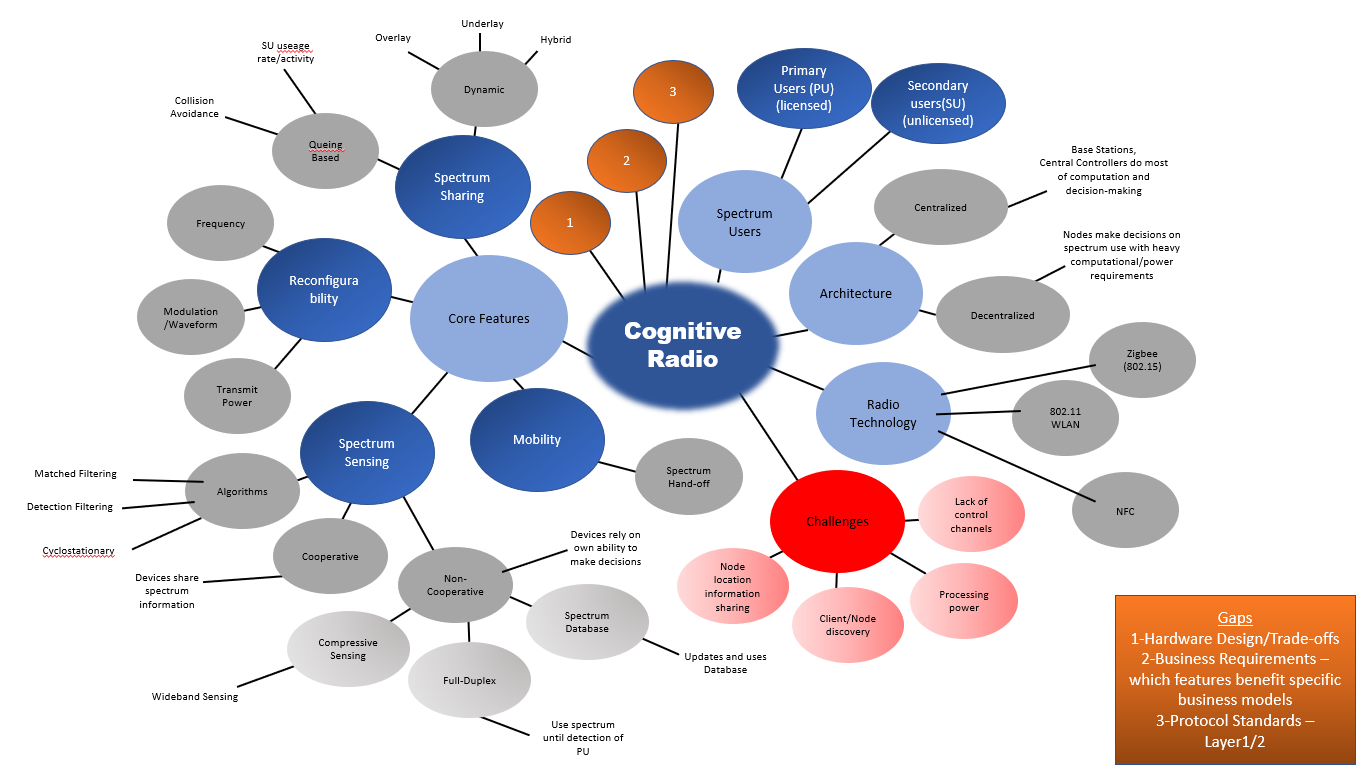
\includegraphics[scale=.50]{TopicMap}
    \caption{Topic Map}
    \label{fig:Topic Map}
       \end{center}
\end{figure}

\newpage
\bibliographystyle{ieeetr}
\bibliography{Bib.bib}
\end{document}
